\subsection{Graphs and Networks}
\label{sec:Method:Graphs}
The most common way of describing a network of anything, that could be of accounts on Facebook, the electrical grid, distribution of goods from warehouses to stores etc. is to use a graph.
A graph is a representation of a network that consists of a set of $N$ nodes, the entities whose interactions are being depicted, and edges $E$ which represent said interactions.


\subsubsection{Static Graphs}
\label{sec:Method:Graphs:StaticGraphs}
The most common type of graph is a static graph, providing a representation of the nodes in a network and edges that are static, ie. do not change. 
In the context of this project, the static graph can be seen as a snapshot of a given network at a single point in time.

A static graph representation of the relationships between $N=4$ nodes, you and three friends who do not know each other, could look as the graph presented in figure \ref{fig:StaticGraph}.

\begin{figure}[H]
    \centering
    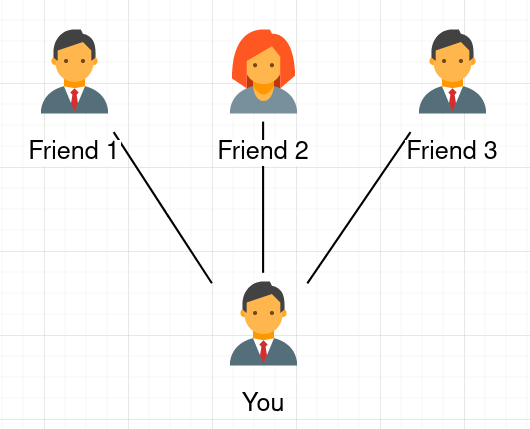
\includegraphics[width=0.5\textwidth]{0_images/static_graph.png}
    \caption{The relationship between you and three friends. You know each one of them, buth they do not know each other.}
    \label{fig:StaticGraph}
\end{figure}
The most common way of representing network information in a machine-interpretable way is with an adjacency matrix $\textbf{A} \in \R^{N \times N}$, \cite{NetworkBarabasi} chapter 2.11.
The adjacency matrix $\textbf{A}$ holds information of whether two given nodes, $u$ and $v$ are connected, having $\textbf{A}_{u,v} = 1$ if a link is present, and $\textbf{A}_{u,v} = 0$ if not.
For the above figure, the appropriate adjacency matrix  with you as the first column/row, friend 1 as the second and so forth, would look as the following:
\begin{equation}
    \textbf{A}_{friends} = \begin{pmatrix}
                - & 1 & 1 & 1\\
                1 & - & 0 & 0\\
                1 & 0 & - & 0\\
                1 & 0 & 0 & -
                \end{pmatrix}
\end{equation}

\subsubsection{Temporally Dynamic Graphs}
\label{sec:Method:Graphs:DynamicGraphs}
Not all networks can be represented by static graphs though, and sometimes having graphs be non-static means that they make for a better representation of the network they are modelling. 

The dynamic aspect differ between graphs, as they can be changing in different dimensions. 
This project focuses entirely on graphs that are dynamic in the temporal dimension, \textit{temporal dynamics graphs}, i.e. they change over time. 
An update happening over time for such a network would be the insertion or deletion of edges or nodes.

A very simple dynamic network, building on the static network example in figure \ref{fig:StaticGraph}, could be visualized by the three static graph representations in figure \ref{fig:DynamicGraph}.

\begin{figure}[H]
    \centering
    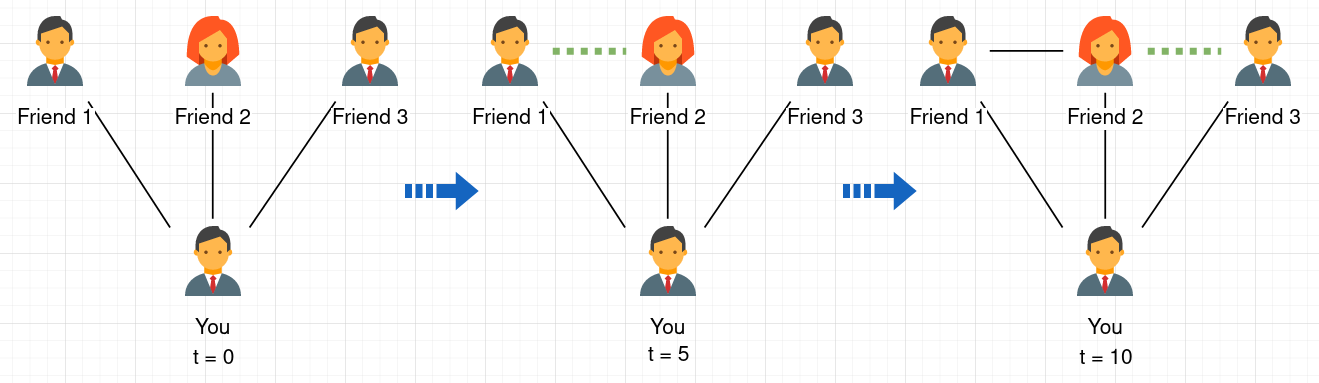
\includegraphics[width=\textwidth]{0_images/dynamic_graph2.png}
    \caption{The dynamic relationship between you and three friends, changing from time $t=0$, to time $t=5$ and lastly $t=10$. Between each time, the friends get to know each other, and the graph hence changes over time.}
    \label{fig:DynamicGraph}
\end{figure}
This kind of representation, called \textit{Discrete-time dynamic graphs} \cite{Rossi2020TEMPORALGRAPHS} (p. 2), entails that the dynamics of the network are presented as snapshots, ie. static graph representations, for different time points throughout the dynamic network.
Using this representation approach, the adjacency matrix representation would hence also be three separate matrices, each representing the time points $t= [0,5,10]$ 

\begin{equation}
    \textbf{A}_{t=0} = \begin{pmatrix}
                - & 1 & 1 & 1\\
                1 & - & 0 & 0\\
                1 & 0 & - & 0\\
                1 & 0 & 0 & -
                \end{pmatrix}, \hspace{10pt}
    \textbf{A}_{t=5} = \begin{pmatrix}
                - & 1 & 1 & 1\\
                1 & - & 1 & 0\\
                1 & 1 & - & 0\\
                1 & 0 & 0 & -
                \end{pmatrix}, \hspace{10pt}
    \textbf{A}_{t=10} = \begin{pmatrix}
                - & 1 & 1 & 1\\
                1 & - & 1 & 0\\
                1 & 1 & - & 1\\
                1 & 0 & 1 & -
                \end{pmatrix}, \hspace{10pt}
\end{equation}

Another approach to representing networks with temporal dynamics is what is called \textit{continious-time dynamic graphs} \cite{Rossi2020TEMPORALGRAPHS} (p. 2).
With this approach, the dynamic graphs is represented as timed lists of $n$ events, in which the link between two nodes $u$ and $v$ at a point in time $t$ is written as a tuple $(u, v, t)$.
With this representation, the example given in figure \ref{fig:DynamicGraph} would be written as the following:

\begin{equation}
    \begin{bmatrix}
            (you, friend1, 0)\\
            (you, friend2, 0)\\
            (you, friend3, 0)\\
            (you, friend1, 5)\\
            (you, friend2, 5)\\
            (you, friend3, 5)\\
            (friend1, friend2, 5)\\            
            (you, friend1, 10)\\
            (you, friend2, 10)\\
            (you, friend3, 10)\\
            (friend1, friend2, 10)\\
            (friend2, friend3, 10)\\
            \end{bmatrix}
\end{equation}
\\
When talking about the graphs of a dynamic network, this project refers to graphs that are subject to a sequence of \textit{updates} over time, and hence continuous-time dynamic graphs are appropriate in their representation. 




